\section{Multiple Linear Regression}\label{sc:multipleLinearRegression}

\subsection{Theory}
Simple Linear Regression is used to make linear models of data. It has a response Y on the basis of a single predictor variable X. We can write it as:
\begin{align}\label{fo:simpleLinearRegression}
Y = \beta_0 + \beta_1 X + \epsilon
\end{align}
$ \beta_0 + \beta_1 $ are unknown and to get a response, we must use data to estimate the coefficients.$(x_1, y_1)$, $(x_2, y_2)$,\dots, $(x_n, y_n)$ represent n observation pairs, each of which consists of a measurement of X and a measurement of Y. The drawback of this method is that only a single predictor variable is used and often have more.
 In cases where we want examined the relationship between multiple predictor variables we use Multiple Linear Regression. The model takes the following form:
\begin{align}\label{fo:multipleLinearRegression}
Y = \beta_0 + \beta_1 X_1 + \ldots + \beta_n X_n + \epsilon
\end{align}
To obtain the estimated Coefficients in the model we use the least squares method to minimize the sum of squared residuals. We pick $\hat{\beta_0}, \hat{\beta_1}, ... \hat{\beta_p}$ to to minimize the sum of squared residuals.
\begin{align}\label{fo:rss}
RSS = \sum (y - \hat{y})^2 = \sum( y_i - \hat{\beta_0} - \hat{\beta_1}x_{i1} - \hat{\beta_2}x_{i2} - \ldots - \hat{\beta_p}x_\textit{i}p )^2
\end{align}
To evaluated the model we can use RSE (residual standard error). This is done by meaning and rooting the result of the RSS. The outcome of the formula is the average amount that the response will deviate from the regression line. This is also known as an estimate of the error, $\epsilon$, in the Standard Linear Regression formula (\ref{fo:simpleLinearRegression}) stated earlier in this chapter:
\begin{align}\label{fo:rse}
RSE = \sqrt{\dfrac{1}{n-2}\cdot RSS}
\end{align}


\subsection{Results}
The lab 3.6.2 and 3.6.3 are using linear and multiple regression respectively, to test if there is a dependency between any of the values. The dataset tested on is housing values in suburbs of Boston\footnote{https://raw.github.com/vincentarelbundock/Rdatasets/master/csv/MASS/Boston.csv}.

\subsubsection*{LAB 3.6.2}
In the lab 3.6.2 was made a linear regression on MEDV (\textit{Median value of owner-occupied homes in \$1000's}) and LSTAT (\textit{Lower status of the population}). Starting off by making a scatter plot of the data to observe how the data look compared to each other.

\begin{figure}[h]
	\centering
	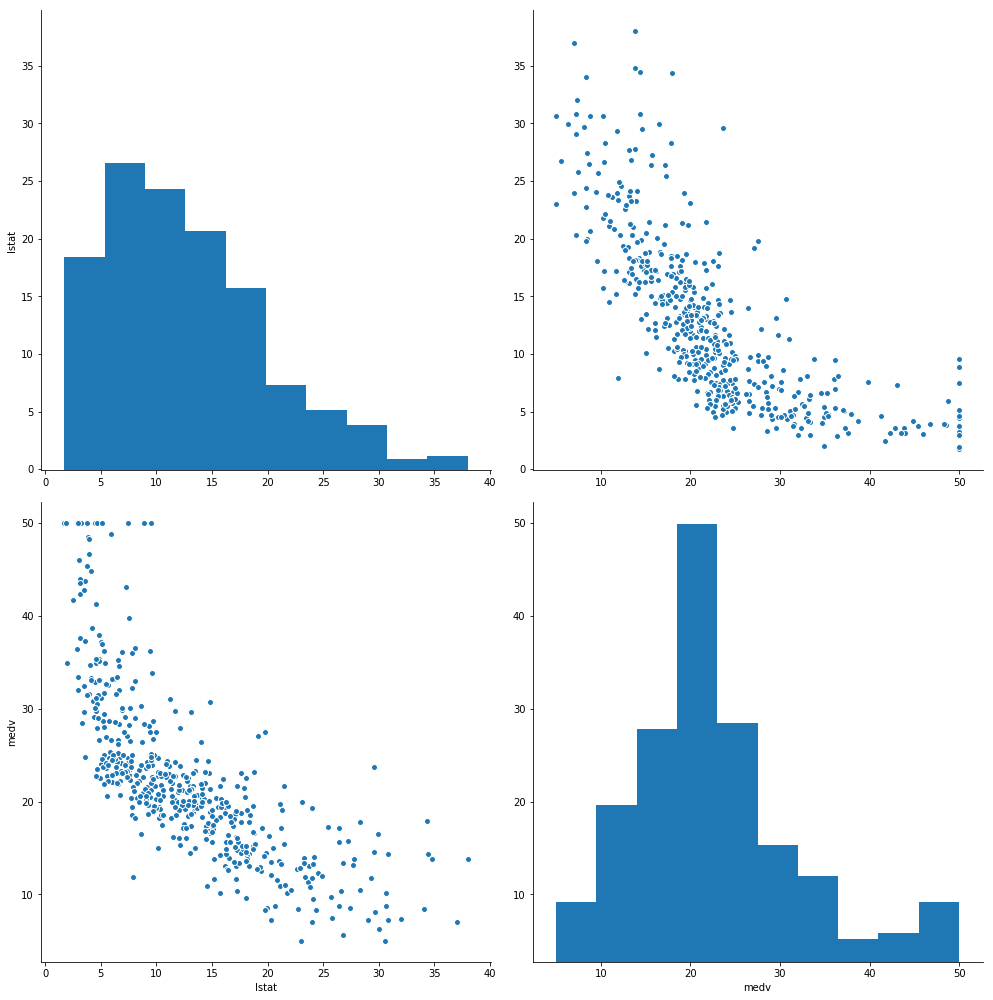
\includegraphics[scale=0.4, trim=0 0 0 500, clip=true]{regression/multipleLinearRegression/fig/bostonPairplotMdevLstat.png}
	\caption{Relationship between the feature and the response using scatter plots.}
	\label{fig:bostonPairplotMdevLstat}
\end{figure}

The Figure \ref{fig:bostonPairplotMdevLstat} shows that making a simple linear regression on these data, might be stretching it, but to be sure the linear regression were made. Resulting in the following output:

\noindent\textit{Intercept: 34.5538408794\\
Coefficients: [-0.95004935]\\
Variance score: 0.54\\}

The variance score is 0.54, which says that the simple linear fit on these data isn't very precise. Making a scatter plot will help to visualize this observation.

\begin{figure}[h]
	\centering
	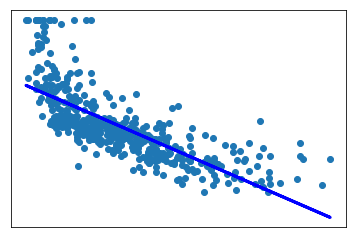
\includegraphics[scale=0.6]{regression/multipleLinearRegression/fig/bostonScatterplotMdevLstatLinreg.png}
	\caption{Relationship between the feature and the response using scatter plots, with linear fit.}
	\label{fig:bostonScatterplotMdevLstatLinreg}
\end{figure}

As the Figure \ref{fig:bostonScatterplotMdevLstatLinreg} shows both data points at the start and at the end is far away from the linear fit. The conclusion on both the variance and the observed data that there is some evidence of non-linearity.

\subsubsection*{LAB 3.6.3}
The lab 3.6.3 continuous working on the MDEV (Median value of owner-occupied homes in $\$1000's$) and LSTAT (\% lower status of the population) data, but also include AGE (\textit{proportion of owner-occupied units built prior to 1940}). First step is to make scatter plot of the data in order to visuals and observe the datasets compared to each other. This time taking a step further and get an approximate of the linear regression fit, as seen on Figure \ref{fig:bostonPairplotMdevLstatAge}.

\begin{figure}[h]
	\centering
	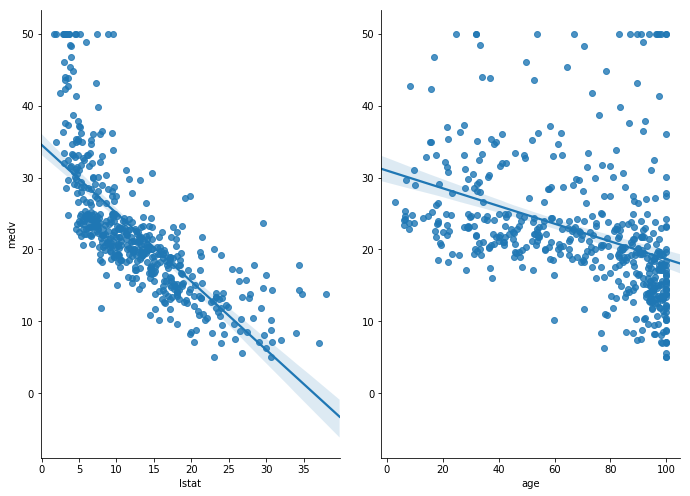
\includegraphics[scale=0.4]{regression/multipleLinearRegression/fig/bostonPairplotMdevLstatAge.png}
	\caption{Relationship between the feature and the response using scatterplots.}
	\label{fig:bostonPairplotMdevLstatAge}
\end{figure}

The linear regression were made on the features and the response. Resulting in the following output:

\noindent\textit{Intercept: 33.2227605318\\
	Coefficients: [('lstat', -1.0320685641826013), ('age', 0.034544338571646085)]\\
	Variance score: 0.55\\}

Once again the variance score is too low to assume linearity and therefore the conclusion is that there some evidence of non-linearity.

\subsection{Conclusion}
Linear regression is a good way of observing a dataset and checking if there is a linear or non-linear dependency between any of the data. However it is a very simple regression and has a hard time modeling complex data, where the data is not linearly correlated. Data without a linear correlation will result in a high variance, and a high deviation from the fit.